\begin{exercício}{Condições de contorno para meios lineares}{exercício2}
    Na interface entre dois meios dielétricos, o campo elétrico deve necessariamente ser consistente com as condições de contorno que você resumiu no problema anterior. Assim, considere uma interface genérica entre dois meios \emph{lineares}, como mostra a figura abaixo. As constantes \(\epsilon_1\) e \(\epsilon_2\) correspondem às permissividades elétricas de cada um dos meios e os campos elétricos estão indicados.

    \begin{center}
        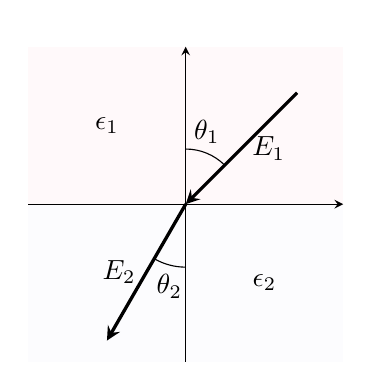
\begin{tikzpicture}
            \fill[Lavender!10] (-2,-2) rectangle (2,0);
            \fill[Pink!10] (-2,0) rectangle (2,2);
            % Axes
            \draw[-stealth] (-2,0) -- (2,0) node[right] {};
            \draw[-stealth] (0,-2) -- (0,2) node[above] {};

            % Arrows for E1 and E2 using polar coordinates
            \draw[very thick, stealth-] (0,0) -- +(45:2) node[midway,right] {$\vetor{E}_1$};
            \draw[very thick, -stealth] (0,0) -- +(-120:2) node[midway,left] {$\vetor{E}_2$};

            % Theta1 angle
            \draw (0,0.7) arc[start angle=90,end angle=45,radius=0.7] node[midway,above] {\(\theta_1\)};

            % Theta2 angle
            \draw (0,-0.8) arc[start angle=270,end angle=240,radius=0.8] node[midway, below] {\(\theta_2\)};

            % Labels for permittivities
            \node at (-1,1) {$\epsilon_1$};
            \node at (1,-1) {$\epsilon_2$};
        \end{tikzpicture}
    \end{center}

    Prove que \(\epsilon_2 \tan{\theta_1} = \epsilon_1 \tan{\theta_2}\).
\end{exercício}
\begin{proof}[Resolução]

\end{proof}
